% =============================================================================
%  Section: Kinematic Binning
%  H1 Charged-Hadron SIDIS High-Q^2 Analysis Note
% =============================================================================
\section{Kinematic Binning}
\label{sec:binning}

The current high-$\Qsq$ analysis uses the binning summarized in Table~\ref{tab:binning:z005-contract}.  The
corresponding inclusive DIS measurement phase space in the $(x_{\mathrm{Bj}},
\Qsq)$ plane is shown in Fig.~\ref{fig:binning:kinematic-plane}.  The published
$\pTh$ bins are coarser than the reconstruction-level $\pTh$ bins used in the
response matrix.

\begin{figure}[t]
\centering
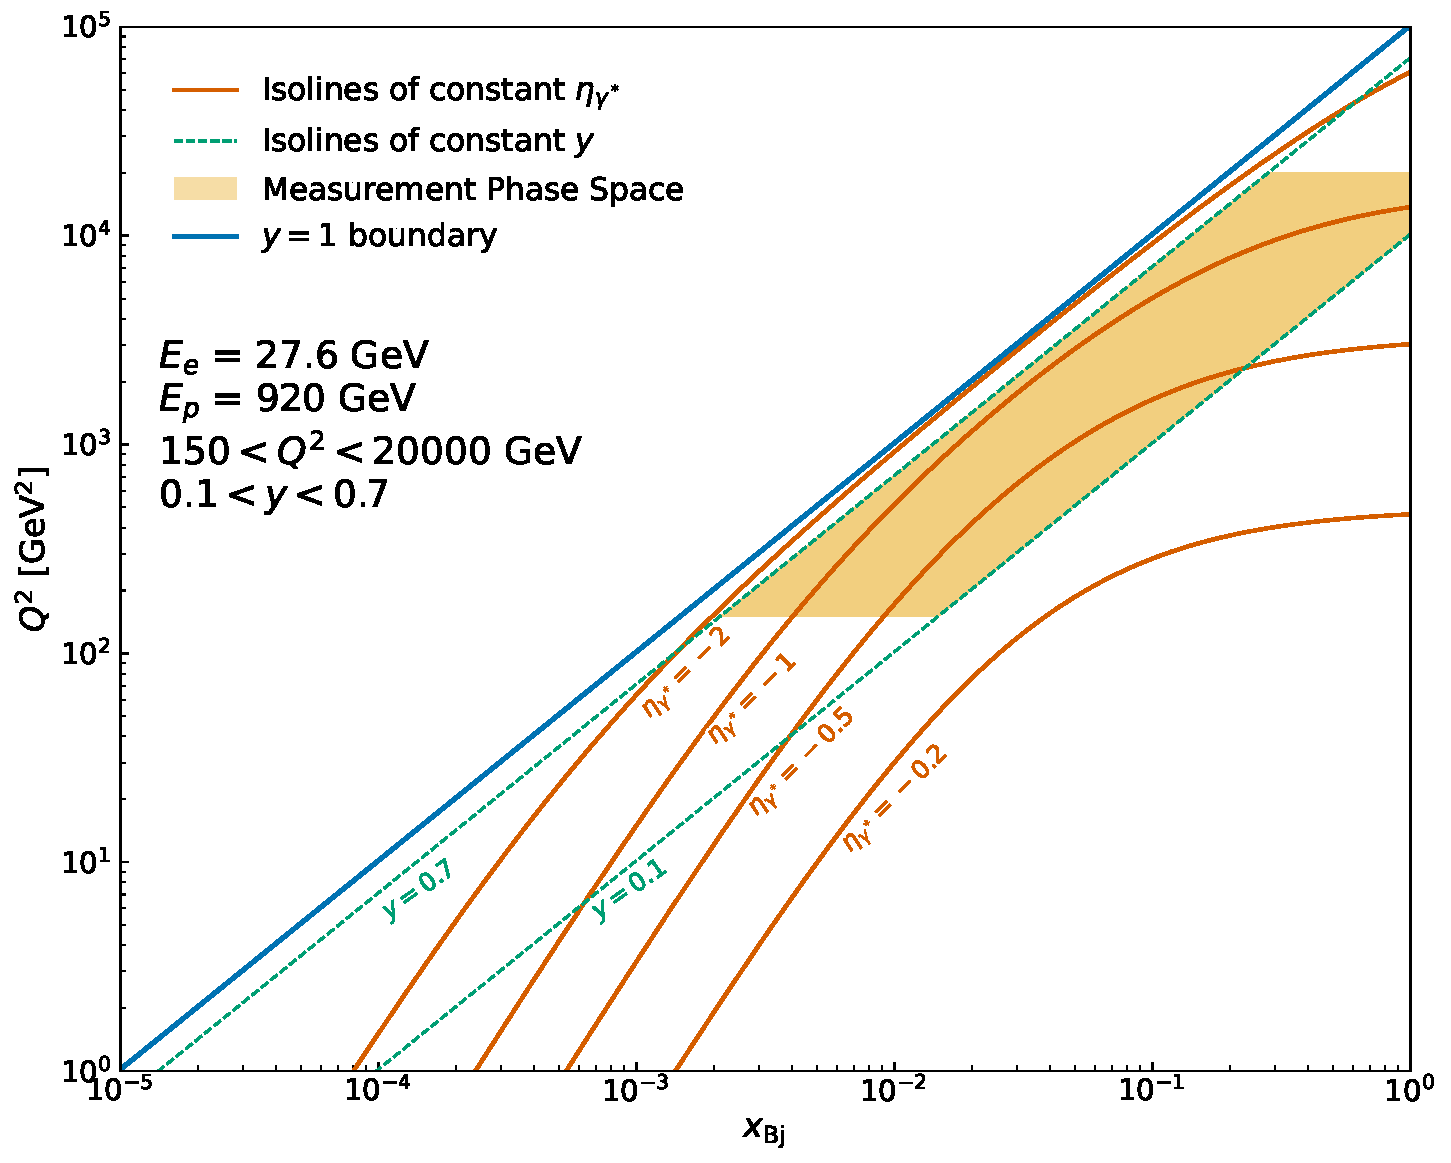
\includegraphics[width=0.82\textwidth]{figures/HERA_xQ2_virtual_photon_eta.pdf}
\caption{Measurement phase space in the $(x_{\mathrm{Bj}},\Qsq)$ plane for the
high-$\Qsq$ charged-hadron SIDIS analysis.  The shaded region indicates the
measurement phase space, and the orange curves show isolines of constant
$\eta_{\gamma^{*}}$ for the virtual photon.  Constant-$y$ isolines and the
$y=1$ boundary are shown for orientation.}
\label{fig:binning:kinematic-plane}
\end{figure}

\begin{table}[h]
\centering
\small
\begin{tabular}{lp{9.3cm}}
\toprule
Quantity & Contract \\
\midrule
$z$ edges (7 bins) & $[0.0,0.05,0.1,0.2,0.3,0.5,0.7,1.0]$ \\
Published $\pTh$ edges (5 bins) & $[0.0,0.5,1.0,2.0,4.0,8.0]~\GeV$ \\
$(\Qsq,x)$ intervals (7 cells) & $150<\Qsq<300~\GeVsq$: $0.0021<x<0.0071$ and $0.0071<x<0.030$; $300<\Qsq<700~\GeVsq$: $0.0042<x<0.016$ and $0.016<x<0.069$; $700<\Qsq<1500~\GeVsq$: $0.0099<x<0.034$ and $0.034<x<0.150$; $1500<\Qsq<20000~\GeVsq$: $0.021<x<1.0$\footnotemark \\
Published bins & 245 per charge; 490 total \\
Response and data vectors & Response matrix $(491,246)$ per charge; data-vector length 980 \\
\bottomrule
\end{tabular}
\caption{Validated binning and response contract for the current high-$\Qsq$
analysis release.  The reconstruction-level $\pTh$ binning is deliberately
finer than the published binning.}
\label{tab:binning:z005-contract}
\end{table}
\footnotetext{The internal binning container carries $x_{\max}=1.5$ only to catch migrations; it is not part of the published binning.}

The binning is charge separated: every published bin appears once for $\hplus$
and once for $\hminus$.  The generator-side published grid contains 245 bins per
charge.  

The reconstructed-side binning used in the migration matrix is twice as fine in $\pTh$, using the ten-bin edge set given in Sec.~\ref{sec:selection:final-tracks}, with 490 reconstructed bins total per
charge.  This permits migrations to be modeled before the result is unfolded
back to the 245-bin published grid per charge. An additional row and column in
the stored migration matrix is used for handling fakes and misses.

